\subsection{エンド}\label{chap-7.5-end}
  定自然変換$\natf{\varDelta f}{\varDelta A}{\varDelta B}{C}{D}$は、圏$\cat{C}$の任意の対象$C$に対して$(\varDelta f)_C=f$となる自然変換であった。一方で定関手$\varDelta A$でも$\varDelta A(C)=A$が成り立つが、この性質は定写像$\mor{\varDelta A}{\obj{C}}{\obj{D}}$によって定義されている。定自然変換と違い、関手に対象を適用する操作は対象関数で与えられているが、自然変換には与えられておらず、自然変換の成分を取る操作は写像によって定義したわけではない。\\
  自然変換を対象によって添え字付けられた射の束、と定義するのでは無く、射集合の何らかの操作によって定義できると考えたかもしれない。これは実際にエンドと呼ばれる一種の普遍性を用いることで、自然変換を再定義することができる。\\
  \begin{prop}[自然変換の普遍性]\label{prop-university-of-nat}
    圏$\cat{C}$の任意の対象$C$に対して$\cat{Set}$の射$\mor{\lambda_C}{\arset{\funccat{C}{D}}{F}{G}}{\arset{D}{FC}{GC}}$が存在し、$\cat{C}$の任意の射$\mor{f}{A}{B}$に対して、\[\arset{D}{FA}{Gf}\circ\lambda_A=\arset{D}{Ff}{GB}\circ\lambda_B\]を満たす。
    
    \begin{center}
      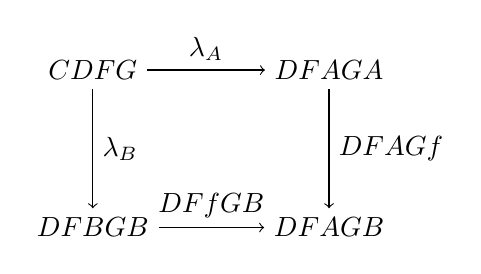
\begin{tikzpicture}[auto]
        \node (FG) at (0, 0) {$\arset{\funccat{C}{D}}{F}{G}$};
        \node (FAGA) at (3, 0) {$\arset{D}{FA}{GA}$};
        \node (FBGB) at (0, -2) {$\arset{D}{FB}{GB}$};
        \node (FAGB) at (3, -2) {$\arset{D}{FA}{GB}$};

        \draw[->] (FG) to node{$\lambda_A$}(FAGA);
        \draw[->] (FG) to node{$\lambda_B$}(FBGB);
        \draw[->] (FAGA) to node{$\arset{D}{FA}{Gf}$}(FAGB);
        \draw[->] (FBGB) to node{$\arset{D}{Ff}{GB}$}(FAGB);

      \end{tikzpicture}
    \end{center}
    
    またある対象$X$に対しても任意の対象$C$に対する$\mor{\mu_C}{\arset{\funccat{C}{D}}{F}{G}}{\arset{D}{FC}{GC}}$が存在し、\[\arset{D}{FA}{Gf}\circ\mu_A=\arset{D}{Ff}{GB}\circ\mu_B\]を満たすのであれば、
    \begin{center}
      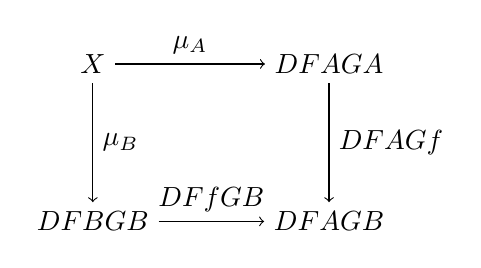
\begin{tikzpicture}[auto]
        \node (FG) at (0, 0) {$X$};
        \node (FAGA) at (3, 0) {$\arset{D}{FA}{GA}$};
        \node (FBGB) at (0, -2) {$\arset{D}{FB}{GB}$};
        \node (FAGB) at (3, -2) {$\arset{D}{FA}{GB}$};

        \draw[->] (FG) to node{$\mu_A$}(FAGA);
        \draw[->] (FG) to node{$\mu_B$}(FBGB);
        \draw[->] (FAGA) to node{$\arset{D}{FA}{Gf}$}(FAGB);
        \draw[->] (FBGB) to node{$\arset{D}{Ff}{GB}$}(FAGB);

      \end{tikzpicture}
    \end{center}
    任意の対象$C$に対して$\mu_C=\lambda_C\circ h$を満たすような射$\mor{h}{X}{\arset{\funccat{C}{D}}{F}{G}}$が一意に存在する。すなわち、$\mu_C=\lambda_C\circ h'$を満たすような$h'$が存在すれば、$h'=h$が成り立つ。
    \begin{center}
      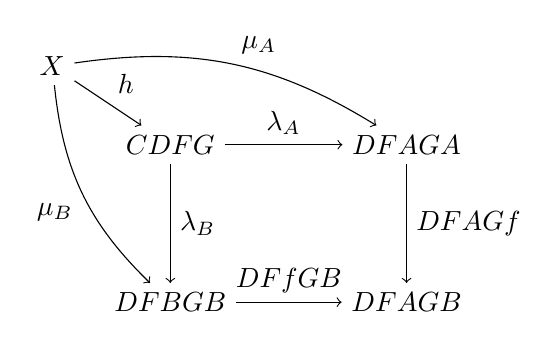
\begin{tikzpicture}[auto]
        \node (FG) at (0, 0) {$\arset{\funccat{C}{D}}{F}{G}$};
        \node (X) at (-1.5, 1) {$X$};
        \node (FAGA) at (3, 0) {$\arset{D}{FA}{GA}$};
        \node (FBGB) at (0, -2) {$\arset{D}{FB}{GB}$};
        \node (FAGB) at (3, -2) {$\arset{D}{FA}{GB}$};

        \draw[->] (FG) to node{$\lambda_A$}(FAGA);
        \draw[->] (X) to node{$h$}(FG);

        \draw[->] (FG) to node{$\lambda_B$}(FBGB);
        \draw[->,bend left = 20] (X) to node{$\mu_A$}(FAGA);
        \draw[->,bend right = 20] (X) to node[swap]{$\mu_B$}(FBGB);
        \draw[->] (FAGA) to node{$\arset{D}{FA}{Gf}$}(FAGB);
        \draw[->] (FBGB) to node{$\arset{D}{Ff}{GB}$}(FAGB);

      \end{tikzpicture}
    \end{center}
  \end{prop}
  \begin{proof}
    まず任意の対象$C$に対する$\cat{Set}$の射$\mor{\lambda_C}{\arset{\funccat{C}{D}}{F}{G}}{\arset{D}{FC}{GC}}$を定義する。\\
    任意の自然変換$\nat{\alpha}{F}{G}$に対して$\lambda_C(\alpha)=\alpha_C$とする。任意の自然変換はある対象に対する成分をただ一つ持つから、この操作は写像であり、$\cat{Set}$の射である。すると、
    \begin{align*}
      \arset{D}{FA}{Gf}\circ\lambda_A(\alpha)&=\arset{D}{FA}{Gf}(\alpha_A)&\text{($\lambda$の定義)}\\
      &=Gf\circ\alpha_A&\text{(射写像の定義)}\\
      \arset{D}{Ff}{GB}\circ\lambda_B(\alpha)&=\arset{D}{Ff}{GB}(\alpha_B)&\text{($\lambda$の定義)}\\
      &=\alpha_B\circ Ff&\text{(射写像の定義)}
    \end{align*}
  \end{proof}
  であり、$\alpha$の自然性から$Gf\circ\alpha_A=\alpha_B\circ Ff$が成り立つ。よって$\arset{D}{FA}{Gf}\circ\lambda_A=\arset{D}{Ff}{GB}\circ\lambda_B$を満たす。\\
  この等式では自然変換の成分が写像で与えられた場合の自然性を射写像を用いて課していることが分かる。\\
  次に射$h$の存在と一意性を示そうと思う。そこでまずは任意の対象$X$に終対象$1$を当てはめて考える。射$\mor{\mu_C}{1}{\arset{D}{FC}{GC}}$は射$\mor{\mu_A}{FA}{GA}$であり、任意の対象$C$に対して存在する。更に仮定より$\arset{D}{FA}{Gf}\circ\mu_A=\arset{D}{Ff}{GB}\circ\mu_B$が成り立つ。
  \begin{align*}
    \arset{D}{FA}{Gf}\circ\mu_A&=\arset{D}{Ff}{GB}\circ\mu_B\\
    \arset{D}{FA}{Gf}(\mu_A)&=\arset{D}{Ff}{GB}(\mu_B)&\text{(元と終対象からの射の同一視)}\\
    Gf\circ\mu_A&=\mu_B\circ Ff&\text{(射写像の定義)}
  \end{align*}
  よって自然変換の定義より、$\mu_C$は対象$C$成分であることが分かる。この自然変換を$\nat{\mu}{F}{G}$とすると、$\mu$は$\arset{\funccat{C}{D}}{F}{G}$の元である。すなわち$\mor{\mu}{1}{\arset{\funccat{C}{D}}{F}{G}}$と表せる。ここで$h=\mu$とすると$\lambda$は成分を取る写像であったから、$\mu_C=\lambda_C(\mu)=\lambda_C\circ\mu=\lambda_C\circ h$が成り立つ。
  \begin{center}
    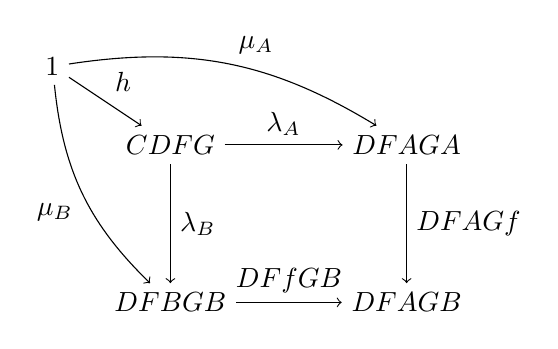
\begin{tikzpicture}[auto]
      \node (FG) at (0, 0) {$\arset{\funccat{C}{D}}{F}{G}$};
      \node (X) at (-1.5, 1) {$1$};
      \node (FAGA) at (3, 0) {$\arset{D}{FA}{GA}$};
      \node (FBGB) at (0, -2) {$\arset{D}{FB}{GB}$};
      \node (FAGB) at (3, -2) {$\arset{D}{FA}{GB}$};

      \draw[->] (FG) to node{$\lambda_A$}(FAGA);
      \draw[->] (X) to node{$h$}(FG);

      \draw[->] (FG) to node{$\lambda_B$}(FBGB);
      \draw[->,bend left = 20] (X) to node{$\mu_A$}(FAGA);
      \draw[->,bend right = 20] (X) to node[swap]{$\mu_B$}(FBGB);
      \draw[->] (FAGA) to node{$\arset{D}{FA}{Gf}$}(FAGB);
      \draw[->] (FBGB) to node{$\arset{D}{Ff}{GB}$}(FAGB);
    \end{tikzpicture}
  \end{center}
  一意性に関しても、$\mu_C=\lambda_C\circ h'$であるような$h'$が存在したとしても、$\mu_C={h'}_C$であり、自然変換の定義から$h'=\mu=h$が成り立つ。\\
  次に対象$1$を任意の対象$X$に拡張しよう。$X$の任意の元$x$に対し$\mu_C(x)$はある自然変換の$C$成分である。上記の議論から自然変換$h(x)_C=\mu_C(x)$であるため、自然変換$h(x)$は任意の$x$に対して一意に存在することになる。

  \begin{center}
    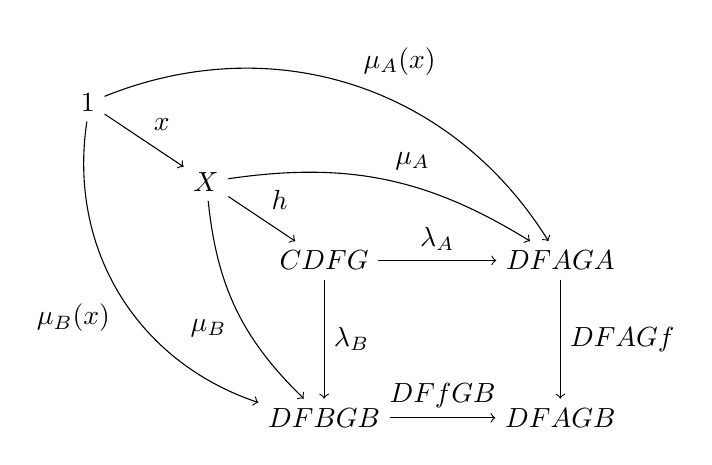
\begin{tikzpicture}[auto]
      \node (FG) at (0, 0) {$\arset{\funccat{C}{D}}{F}{G}$};
      \node (X) at (-1.5, 1) {$X$};
      \node (1) at (-3, 2) {$1$};
      \node (FAGA) at (3, 0) {$\arset{D}{FA}{GA}$};
      \node (FBGB) at (0, -2) {$\arset{D}{FB}{GB}$};
      \node (FAGB) at (3, -2) {$\arset{D}{FA}{GB}$};
      \draw[->] (FG) to node{$\lambda_A$}(FAGA);
      \draw[->] (X) to node{$h$}(FG);
      \draw[->] (1) to node{$x$}(X);
      \draw[->] (FG) to node{$\lambda_B$}(FBGB);
      \draw[->,bend left = 20] (X) to node{$\mu_A$}(FAGA);
      \draw[->,bend right = 20] (X) to node[swap]{$\mu_B$}(FBGB);
      \draw[->,bend left = 40] (1) to node{$\mu_A(x)$}(FAGA);
      \draw[->,bend right = 40] (1) to node[swap]{$\mu_B(x)$}(FBGB);
      \draw[->] (FAGA) to node{$\arset{D}{FA}{Gf}$}(FAGB);
      \draw[->] (FBGB) to node{$\arset{D}{Ff}{GB}$}(FAGB);
    \end{tikzpicture}
    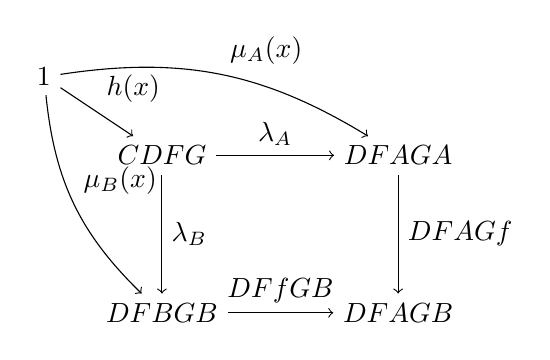
\begin{tikzpicture}[auto]
      \node (FG) at (0, 0) {$\arset{\funccat{C}{D}}{F}{G}$};
      \node (X) at (-1.5, 1) {$1$};
      \node (FAGA) at (3, 0) {$\arset{D}{FA}{GA}$};
      \node (FBGB) at (0, -2) {$\arset{D}{FB}{GB}$};
      \node (FAGB) at (3, -2) {$\arset{D}{FA}{GB}$};
      \draw[->] (FG) to node{$\lambda_A$}(FAGA);
      \draw[->] (X) to node{$h(x)$}(FG);
      \draw[->] (FG) to node{$\lambda_B$}(FBGB);
      \draw[->,bend left = 20] (X) to node{$\mu_A(x)$}(FAGA);
      \draw[->,bend right = 20] (X) to node{$\mu_B(x)$}(FBGB);
      \draw[->] (FAGA) to node{$\arset{D}{FA}{Gf}$}(FAGB);
      \draw[->] (FBGB) to node{$\arset{D}{Ff}{GB}$}(FAGB);
    \end{tikzpicture}
  \end{center}